\documentclass[11pt,a4paper]{article}
\usepackage[margin=2.2cm]{geometry}
\usepackage{amsmath,amssymb}
\usepackage{siunitx}
\usepackage{booktabs}
\usepackage{xcolor}
\usepackage{microtype}
\usepackage{enumitem}
\usepackage{tcolorbox}
\usepackage{graphicx}
\definecolor{ink}{HTML}{14231B}\definecolor{accent}{HTML}{0F3D2A}
\tcbuselibrary{skins}
\newtcolorbox{key}{colback=accent!6,colframe=accent,boxrule=0.6pt,arc=2pt,left=6pt,right=6pt,top=4pt,bottom=4pt}
\sisetup{per-mode=symbol,group-separator={\,}}
\setlength{\parindent}{0pt}\setlength{\parskip}{6pt}
\renewcommand{\arraystretch}{1.25}

\title{\textbf{Slide 12: board and layout}\\\large A 125 $\times$ 21.5 mm strip that fits adjacent PMOD ports}
\author{ADS7057 test board v3 \quad ---\quad study notes}\date{}
\begin{document}\maketitle\vspace{-1.2em}
\section{The floor plan}
\begin{center}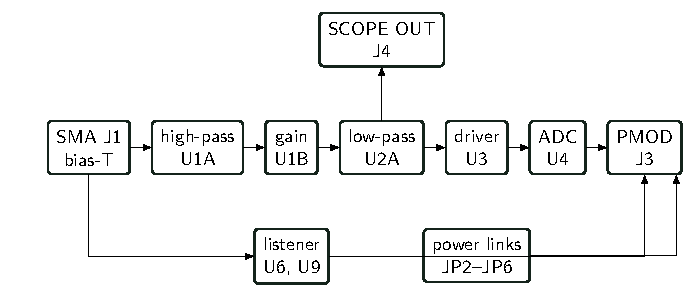
\includegraphics[width=0.98\textwidth]{s12_circuit.pdf}\end{center}
The signal runs from the SMA on the left to the PMOD on the right. The listener, the power links and SCOPE OUT sit around that line.

\section{The board in numbers}
\begin{center}\begin{tabular}{lp{10.5cm}}\toprule
Size and stack & 125 $\times$ \SI{21.5}{mm}, two copper layers, \SI{1.6}{mm} FR-4\\
Parts & 105 footprints: 75 SMD, 4 through-hole, 2 mounting holes, 18 test points, 6 solder jumpers\\
Tracks and vias & 886 track segments (836 at \SI{0.2}{mm}, 50 at \SI{0.15}{mm}); 214 vias of \SI{0.6}{mm} with a \SI{0.3}{mm} drill, 119 of them ground stitching\\
Ground & a pour on both layers, tied by the stitching vias\\
Longest analog net & LPF\_OUT, \SI{39}{mm} (it feeds SCOPE OUT and the driver)\\
\bottomrule\end{tabular}\end{center}
The width of \SI{21.5}{mm} comes from the PMOD pitch: ports sit about \SI{22.7}{mm} apart, so several boards fit side by side. A \SI{5}{mm} track delays a signal by about \SI{30}{ps} and a \SI{500}{kHz} wave lasts \SI{2}{\micro s}, so track length does not matter in the analog chain. What matters is where the capacitors sit.

\section{Top view by block}
\begin{center}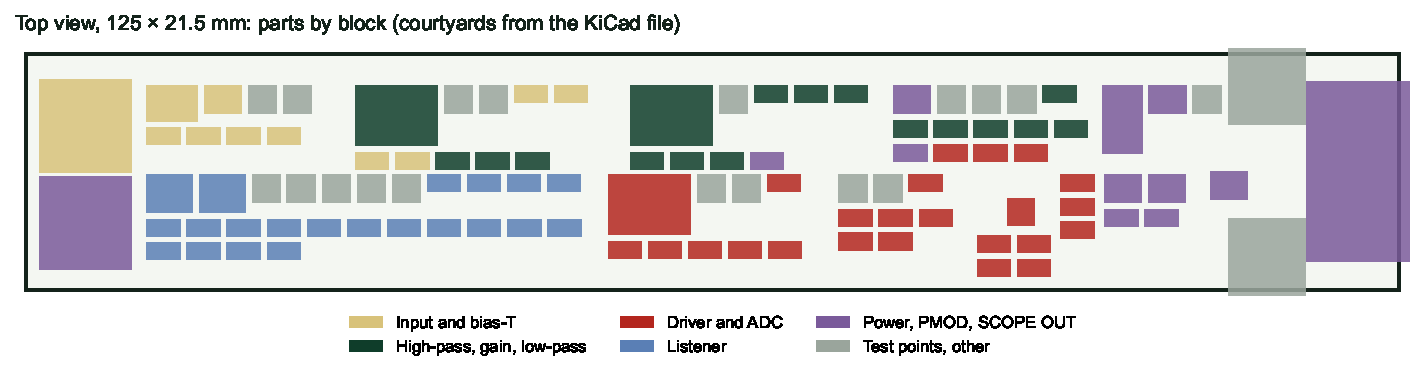
\includegraphics[width=\textwidth]{s12_graph.pdf}\end{center}
Every part belongs to one block. The ADC corner is built tight: the two \SI{10}{\ohm} resistors, the four \SI{100}{pF} capacitors, the supply capacitors and the three \SI{22}{\ohm} resistors all sit around U4. AINP and AINM are 28 and \SI{27}{mm} long, and a \SI{1}{mm} difference is harmless.

\section{What the board offers you on the bench}
\begin{itemize}[leftmargin=1.2em]
\item Test points after every stage: TP3 SIG\_IN, TP4 HPF\_OUT, TP5 GAIN\_OUT, TP6 LPF\_OUT, TP7 and TP8 driver outputs, TP9 and TP10 ADC inputs, TP11 +3V3, TP12 AVDD, TP13 VMID5, TP14 VOCM, TP15 LST, TP16 WAKE\_N, TP17 BIG\_N, TP18 REFL, TP19 and TP20 ground.
\item Solder jumpers JP1 (head power), JP2 to JP5 (current links), JP6 (PMOD power). SCOPE OUT (J4) copies the signal the ADC sees through $51\,\Omega$.
\end{itemize}

\section{Cost (JLCPCB, economic assembly, shipped to Chile)}
From the calibrated model in \texttt{hw/tools/cost.py} (real quote of 2026-10-12): two ADC boards \$66.84 in goods, five \$117.82; five heads \$40.77. Two ADC boards and five heads with shipping and 19\,\% IVA: about \$141 to \$154. Sixteen cards plus sixteen heads would be about \$383 in goods alone (\$305 and \$79), so a 16-channel system does not fit under \SI{200000}{CLP} (about \$210).

\begin{key}
For 16 channels the same card plugs into a backplane (FMC adapter and two 8-slot modules, \texttt{hw/backplane/}). The card itself does not change.
\end{key}
\end{document}
